\section{Containerization Software}\label{background:containerization}
\todo[inline]{Jos: Better models with examples}
Containerization software isolates processes running on a host from each other.
A process in a container sees a different part of the host system than processes outside of the container. A process inside a container sees a different file system, network interfaces and users than processes outside of the container. Processes inside the container can only see other processes inside the container.

\begin{figure}[ht]
    \centering
    \begin{subfigure}[t]{.45\textwidth}
        \centering
        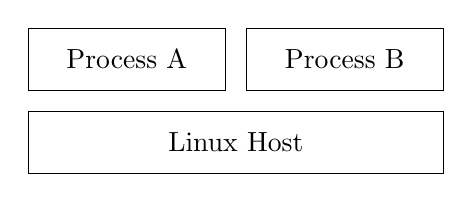
\begin{tikzpicture}[x=0.75pt,y=0.75pt,yscale=-1,xscale=1]
            % Process A Rectangle
            \draw (0,25) -- (95,25) -- (95,55) -- (0,55) -- cycle ;
            \draw (47.5,40) node {Process A};

            % Process B Rectangle
            \draw (105,25) -- (200,25) -- (200,55) -- (105,55) -- cycle ;
            \draw (152.5,40) node {Process B};

            % Host Rectangle
            \draw (0,65) -- (200,65) -- (200,95) -- (0,95) -- cycle ;
            \draw (100, 80) node {Linux Host};
        \end{tikzpicture}
        \caption{Two processes.}\label{subfig:processes}
    \end{subfigure}
    \begin{subfigure}[t]{.45\textwidth}
        \centering
        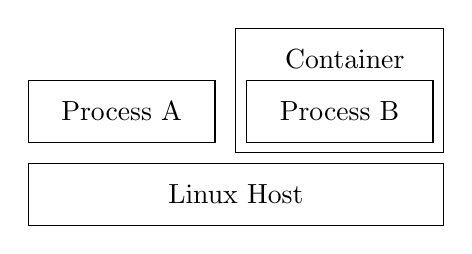
\begin{tikzpicture}[x=0.75pt,y=0.75pt,yscale=-1,xscale=1]
            % Process A Rectangle
            \draw (0,25) -- (90,25) -- (90,55) -- (0,55) -- cycle ;
            \draw (45,40) node {Process A};

            % Process B container Rectangle
            \draw (100,0) -- (200,0) -- (200,60) -- (100,60) -- cycle ;
            \draw (152.5,15) node {Container};

            %% Process B Rectangle
            \draw (105,25) -- (195,25) -- (195,55) -- (105,55) -- cycle ;
            \draw (150,40) node {Process B};

            % Host Rectangle
            \draw (0,65) -- (200,65) -- (200,95) -- (0,95) -- cycle ;
            \draw (100, 80) node {Linux Host};
        \end{tikzpicture}
        \caption{One process in a container.}\label{subfig:container}
    \end{subfigure}
    \caption{}\label{fig:with-without-container}
\end{figure}

If we look at \autoref{fig:with-without-container}, we see two scenarios. \autoref{subfig:processes} is the normal way to run processes. The operating system starts processes that can communicate with other processes. Their view on the file system is the same.
In \autoref{subfig:container} one of the processes runs inside a container. These processes cannot communicate with one another. If Process A looks at the files in \lstinline{/tmp}, it accesses a different part of the file system than when Process B looks at the files in \lstinline{/tmp}\footnote{Access to files on the host has to be explicitly given (as discussed in \autoref{subsection:data-persistence}).}. Process B can not even see that Process A exists.

\medskip

Process A and Process B see such a different part of the host system that to Process B it looks like it is running on a wholly different system.

\subsection{Advantages of Containerization}
\todo[inline]{Jos: better explanation}
Containers can be made into easily deployable packages (called images). These images only contain the necessary files for specific software to run. Other files, libraries and binaries are shared between the host operating system (the system running the container). This allows developers to create lightweight software packages containing only the necessary dependencies.

\medskip

Containers also make it possible to run multiple versions of the same software on one host. Each container can contain a specific version and all the containers run on the same host. Because the containers are isolated from each other, their incompatible dependencies do not pose a problem.

\medskip

For example, if we want to run an instance of Wordpress\footnote{A very popular content management system to build websites with.}, we do not need to install all the Wordpress dependencies. We only need to download the container that the Wordpress developers created, which includes all the necessary dependencies.

Similarly, if we want to move the Wordpress instance from one host to another, we just have to copy the Wordpress database and run the image on the new host. Even if the new host is a completely different operating system.

If we want to test a newer version of Wordpress on the same host, we only have to run the different container on the same host. The incompatible dependencies of the two Wordpress instances are not a problem, because they see different parts of the file system and do not even see each other's processes.

\medskip

The simplicity that containerization brings, makes containerization very popular in software development, maintenance and deployment.

\pagebreak

\subsection{Virtualization}
\todo[inline]{Jos: Hypervisior separate from host in image}
Virtualization is an older, similar technique to isolate software. In virtualization, a whole system is simulated on top of the host (called the hypervisor). This new virtual machine is called a guest. The guest and the host do not share any system resources. This has some advantages. For example, it allows running a completely different guest operating system (e.g.\ a Windows guest on a Linux host).

\begin{figure}[ht]
    \centering
    \begin{subfigure}[t]{.45\textwidth}
        \centering
        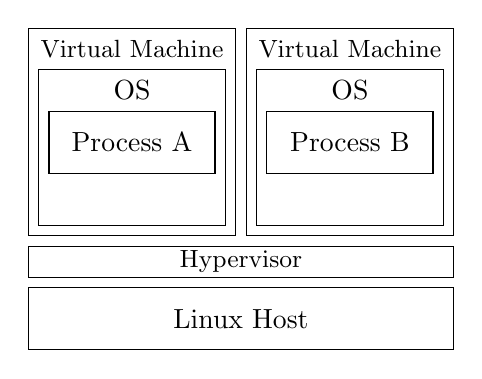
\begin{tikzpicture}[x=0.75pt,y=0.75pt,yscale=-1,xscale=1]
            % VM Process A Rectangle
            \draw (0,0) -- (100,0) -- (100,100) -- (0,100) -- cycle ;
            \draw (50,10) node {{\small Virtual Machine}};

            % OS Process A Rectangle
            \draw (5,20) -- (95,20) -- (95,95) -- (5,95) -- cycle ;
            \draw (50,30) node {OS};

            % Process A Rectangle
            \draw (10,40) -- (90,40) -- (90,70) -- (10,70) -- cycle ;
            \draw (50,55) node {Process A};

            % VM Process B Rectangle
            \draw (105,0) -- (205,0) -- (205,100) -- (105,100) -- cycle ;
            \draw (155,10) node {{\small Virtual Machine}};

            % OS Process B Rectangle
            \draw (110,20) -- (200,20) -- (200,95) -- (110,95) -- cycle ;
            \draw (155,30) node {OS};

            % Process B Rectangle
            \draw (115,40) -- (195,40) -- (195,70) -- (115,70) -- cycle ;
            \draw (155,55) node {Process B};

            % Hypervisor
            \draw (0,105) -- (205,105) -- (205,120) -- (0,120) -- cycle ;
            \draw (102.5,112.5) node {{\small Hypervisor}};

            % Linux Host
            \draw (0,125) -- (205,125) -- (205,155) -- (0,155) -- cycle ;
            \draw (102.5,140) node {Linux Host};
        \end{tikzpicture}
        \caption{Virtual Machines\protect\footnotemark.}
    \end{subfigure}
    \begin{subfigure}[t]{.45\textwidth}
        \centering
         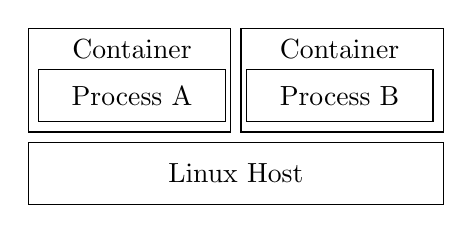
\begin{tikzpicture}[x=0.75pt,y=0.75pt,yscale=-1,xscale=1]
            % Container Process A Rectangle
            \draw (0,0) -- (97.5,0) -- (97.5,50) -- (0,50) -- cycle ;
            \draw (50,10) node {Container};

            % Process A Rectangle
            \draw (5,20) -- (95,20) -- (95,45) -- (5,45) -- cycle ;
            \draw (50,32.5) node {Process A};

            % Container Process B Rectangle
            \draw (102.5,0) -- (200,0) -- (200,50) -- (102.5,50) -- cycle ;
            \draw (150,10) node {Container};

            % Process B Rectangle
            \draw (105,20) -- (195,20) -- (195,45) -- (105,45) -- cycle ;
            \draw (150,32.5) node {Process B};

            % Host Rectangle
            \draw (0,55) -- (200,55) -- (200,85) -- (0,85) -- cycle ;
            \draw (100, 70) node {Linux Host};
        \end{tikzpicture}
        \caption{Containers.}
    \end{subfigure}
    \caption{}
\end{figure}
\footnotetext{Hypervisors can also run on the bare metal. This removes the need for a host OS, which adds security.}

Because containerization software shares many resources with the host, it is a lot faster and more flexible than virtualization. Where virtualization needs to start a whole new operating system, containerization only needs to start a single process.

\subsection{The Impact of Containers on Security}
\todo[inline]{Jos: explain RCE}
A Docker container isolates software from the host, but does not change it. This means that vulnerabilities in software are not affected by Dockerizing that software. However, the impact of those vulnerabilities is decreased, because the vulnerability exists in an isolated environment.

If, for example, there exists a remote code execution (RCE) vulnerability in Wordpress. Running Wordpress in a Docker container does not fix the vulnerability. An attacker is still able to exploit it. But the attacker is far less likely to access the host system, because the exploited software is isolated from the host system because of Docker.

\medskip

Because a container uses the same kernel and resources as the host, a \lstinline{root} exploit (i.e.\ an exploit that allows unprivileged users to escalate their privileges) can be just as effective inside as outside of the container, because the target (e.g.\ the kernel) is the same. CVE--2016--5195(Dirty Cow)\footnote{\url{https://dirtycow.ninja/}} is a good example of an exploit that allows container escapes\cite{Dirty-Cow-Escape}, because it attacks the kernel of the host.
